\documentclass{article}

\usepackage[T1]{fontenc}
\usepackage[utf8]{inputenc}
\usepackage[english]{babel}

\usepackage{amsmath}
\usepackage{siunitx}
\usepackage{hyperref}
\usepackage{listings}
\usepackage{color}
\usepackage{textcomp}
\usepackage{graphicx}
\usepackage{subcaption}
\usepackage[section]{placeins}

\definecolor{matlabgreen}{RGB}{28,172,0}
\definecolor{matlablilas}{RGB}{170,55,241}

\newcommand{\includecode}[1]{\lstinputlisting[caption={\ttfamily #1.m},label={lst:#1}]{matlab/#1.m}}

\newcommand{\inlinecode}[1]{\lstinline[basicstyle=\ttfamily,keywordstyle={}]{#1}}

\author{Riccardo Zanol}
\title{Laboratory 3}

\begin{document}
\lstset{
  language=Matlab,
  basicstyle={\ttfamily \footnotesize},
  breaklines=true,
  morekeywords={true,false,warning,xlim,ylim},
  keywordstyle=\color{blue},
  stringstyle=\color{matlablilas},
  commentstyle={\color{matlabgreen} \itshape},
  numberstyle={\ttfamily \tiny},
  frame=leftline,
  showstringspaces=false,
  numbers=left,
  upquote=true,
}
\maketitle
\section*{Experiment 1}
In the matlab script \inlinecode{ex1.m} each one of the provided
\inlinecode{kodim_*.png} images is mosaiced by
\inlinecode{create_bayer}, that produces an image where the intensity
of each pixel represents only one color component according to the
Bayer pattern ``GRBG'', then the function \inlinecode{demosaic_linear}
is used to linearly interpolate the value of the closest two or four
pixels, depending on the location, to determine the value of each
unknown color component. This function ignores a border of two pixels
around the image and sets it to $(0,0,0)$ to avoid having to handle
this special case in the code.  The script also performs the
demosaicing using the built-in matlab function \inlinecode{demosaic}
which uses a different algorithm, the gradient-corrected bilinear
interpolation, that exploits the correlation between the color
components and corrects the linearly interpolated value of a pixel
with the gradient (of a different color) in that pixel.

After having being demosaiced by each one of the two algorithms the
images are converted into the CIELAB color space to allow them to be
compared to the original images and the mean squared error of the two
algorithms is calculated. The MSE is computed by taking the distance
between each pixel and averaging:
\begin{align*}
  d(i,j) &= \sqrt{\sum_{k=1}^3 \left(A(i,j,k) - B(i,j,k)\right)^2 } \\
  \text{MSE} &= \frac{1}{WH}\sum_{i=0}^H\sum_{j=0}^Wd(i,j)
\end{align*}
where $A(i,j,1) = L(i,j)$, $A(i,j,2) = a(i,j)$ and $A(i,j,3) = b(i,j)$
are the three coordinates in the CIELAB space of the pixel $(i,j)$ of
image $A$. A two pixels wide border is excluded from the comparison
because the function \inlinecode{demosaic_linear} does not perform the
interpolation in this region.  The computed values of the MSE are
shown in Tab.~\ref{tab:mse} where it can be seen that the gradient
correction should improve a lot the quality of the interpolation,
since it halves the MSE.
\begin{table}[h]
  \centering
  \begin{tabular}{ccc}
    Image & Linear interpolation & Gradient corrected interpolation \\
    \hline
    kodim\_01.png & 7.060 & 4.125 \\
    kodim\_05.png & 6.228 & 3.386 \\
    kodim\_13.png & 9.032 & 5.388 \\
    kodim\_19.png & 4.702 & 2.866
  \end{tabular}
  \caption{Mean squared error of the demosaicing algorithms}
  \label{tab:mse}
\end{table}
Unfortunately this is not the case as the gradient correction does
improve a little bit the quality of the reconstructed images, but it
still leaves a lot of noticeable artifacts close to edges and small
details. For example in the detail of image \inlinecode{kodim_19.png},
where both algorithms obtain the smallest value of the MSE, shown in
Fig.~\ref{fig:artifact} there are some colored vertical streaks on the
white fence that are the result of the interpolation.
\begin{figure}[htbp]
  \centering
  \begin{subfigure}{.5\textwidth}
  \centering
  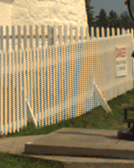
\includegraphics[width=.8\linewidth]{demosaic_kodim19_artifact}
  \caption{\inlinecode{demosaic_linear}}
\end{subfigure}%
\begin{subfigure}{.5\textwidth}
  \centering
  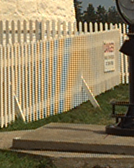
\includegraphics[width=.8\linewidth]{matlab_demosaic_kodim19_artifact}
  \caption{\inlinecode{demosaic}}
\end{subfigure}
\caption{Detail of \inlinecode{kodim_19.png} after the demosaicing}
\label{fig:artifact}
\end{figure}

\section*{Experiment 2}
The matlab script \inlinecode{ex2.m} applies the same two demosaicing
algorithms to some images acquired from a reflex camera. This time,
since it starts from the raw sensor data, it has to perform some
additional steps to get an output that can be compared to the JPEG
files produced by the camera. The script reads the DNG files using the
provided function \inlinecode{read_dng}, which also performs the
linearization and white balancing of the image using the meta-data
stored with it, then it applies the same two demosaicing algorithms
of experiment 1.

The raw data of the image is stored according to a ``RGGB'' Bayer
pattern so the script adds one column of zeros at the beginning and at
the end of the image, in this way it shifts the pattern horizontally
by one pixel and it becomes the ``GRBG'' pattern that the function
\inlinecode{demosaic_linear} expects. The extra columns do not affect
the demosaicing results because this function skips a two pixel wide
border around the image.  The built-in \inlinecode{demosaic} function
could work directly on the ``RGGB'' pattern, but since the two columns
must be added anyway the script uses it in the same way of experiment
1. This function also requires the input pixels to be of type
\inlinecode{uint8} so the image is converted before the demosaicing.

After the demosaicing step, the image is post-processed with the
provided \inlinecode{post_process} function that normalizes the image
intensity and applies a gamma correction.

Comparing the results with the JPEG files produced by the camera it
can be seen that the steps that are skipped in the raw image processing
affect the color, in particular the \inlinecode{post_process} function
does not convert the image from the color space of the camera to
sRGB. As can be seen in Fig.~\ref{fig:chart} the result images appear
to have a much lower contrast than the camera JPEG file.
\begin{figure}[htbp]
  \centering
  \begin{subfigure}{.33\textwidth}
  \centering
  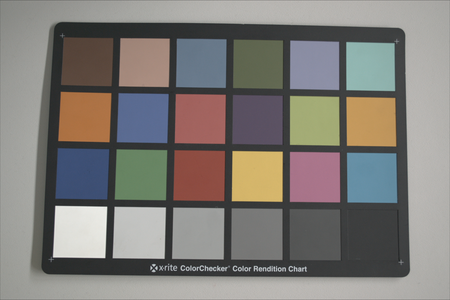
\includegraphics[width=.95\linewidth]{demosaic_macbeth_color_small}
  \caption{\inlinecode{demosaic_linear}}
\end{subfigure}%
\begin{subfigure}{.33\textwidth}
  \centering
  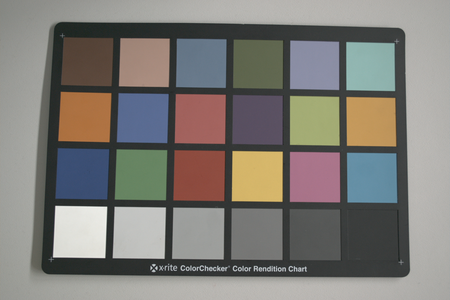
\includegraphics[width=.95\linewidth]{matlab_demosaic_macbeth_color_small}
  \caption{\inlinecode{demosaic}}
\end{subfigure}%
  \begin{subfigure}{.33\textwidth}
  \centering
  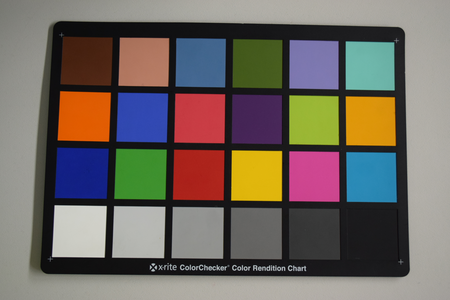
\includegraphics[width=.95\linewidth]{camera_macbeth_color_small}
  \caption{JPEG from the camera}
\end{subfigure}
\caption{Comparison of the color chart}
\label{fig:chart}
\end{figure}
The demosaicing performed by the matlab script also leaves a lot of
artifacts, especially in the dark areas as can be seen from
Fig.~\ref{fig:dark_artifacts}. In this case the linear interpolation
algorithm appears to produce slightly better images than the gradient
corrected one, but they are both very noisy compared to the camera's
processed images.
\begin{figure}[htbp]
  \centering
  \begin{subfigure}{.33\textwidth}
  \centering
  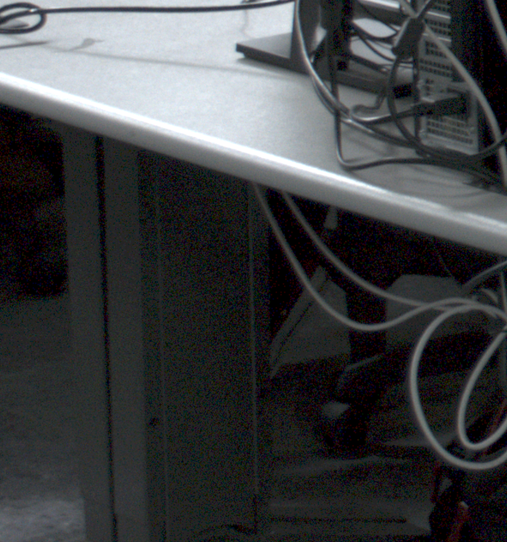
\includegraphics[width=.95\linewidth]{demosaic_students2_detail}
  \caption{\inlinecode{demosaic_linear}}
\end{subfigure}%
\begin{subfigure}{.33\textwidth}
  \centering
  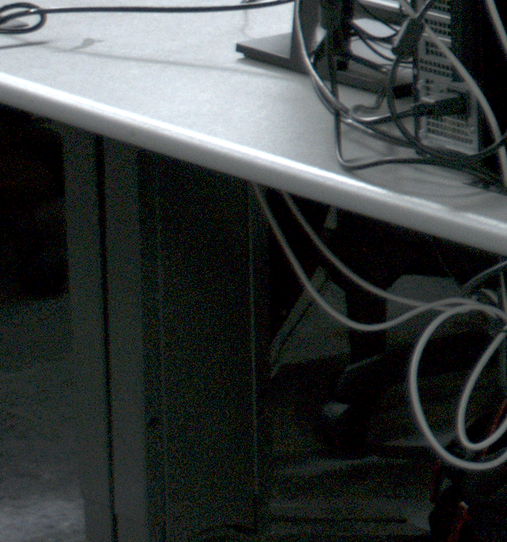
\includegraphics[width=.95\linewidth]{matlab_demosaic_students2_detail}
  \caption{\inlinecode{demosaic}}
\end{subfigure}%
  \begin{subfigure}{.33\textwidth}
  \centering
  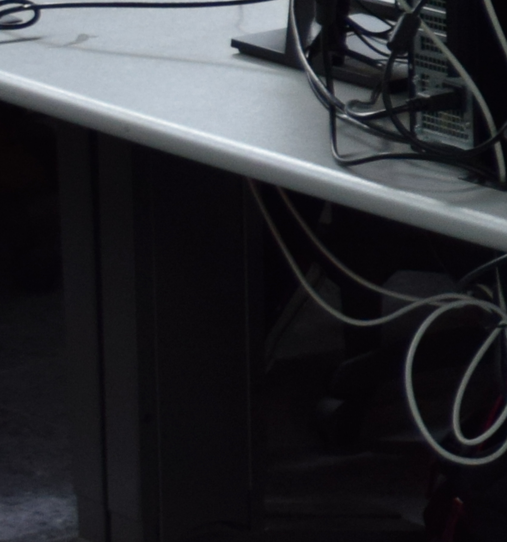
\includegraphics[width=.95\linewidth]{camera_students2_detail}
  \caption{JPEG from the camera}
\end{subfigure}
\caption{Comparison of a detail from \inlinecode{students2.dng}}
\label{fig:dark_artifacts}
\end{figure}
\end{document}
